\documentclass[12pt]{report}

\usepackage[utf8]{inputenc}
\usepackage[T1]{fontenc}
\usepackage[francais]{babel}
\usepackage{setspace}
\usepackage[top=2.5cm,bottom=2.5cm,right=3cm,left=3cm]{geometry}

\usepackage{hyperref}
\usepackage{color}

\usepackage{calc}
\usepackage{pseudocode}

\usepackage{graphicx}

\usepackage{caption}
\captionsetup{figurewithin=none}  
\captionsetup{tablewithin=none}

\AddThinSpaceBeforeFootnotes

\FrenchFootnotes

\title{Rapport de stage}
\author{Antonin Carette}
\date{Compilé le \today}

\begin{document}
\begin{spacing}{1.2}

\maketitle

\tableofcontents

\chapter*{Introduction}

\addcontentsline{toc}{chapter}{Introduction} 

\section{Remerciements}
Je remercie tout d'abord mon tuteur d'Université: M. \textbf{Meftali Samy}, ainsi que mon tuteur en entreprise: M. \textbf{Giraud Mathieu}, pour toute l'attention donnée quant au travail sur le projet, ainsi que sur ce rapport.
\newline
Je remercie ensuite l'équipe Bonsai ainsi que les membres du projet \textit{Vidjil}, pour leur accueil ainsi que leur soutien, recueillis durant les 3 mois de stage.
\newline
Enfin, je tiens mes collèges du bureau 235: M. \textbf{Dufresne Yoann} et M. \textbf{Vrolland Christophe}.

\section{Présentation de l'entreprise, et de l'équipe}

\subsection{Le \textit{L.I.F.L.}}
Le \textit{L.I.F.L.} (Laboratoire d'Informatique Fondamentale de Lille) est un laboratoire Français présent sur le campus de l'Université Lille1, rattaché à l'Institut des Sciences de l'Information et de leurs Interactions (\textit{I.N.S.2.I.}) du \textit{C.N.R.S.} (Centre National de la Recherche Scientifique).
\newline
Il comprend 10 équipes-projets et équipes du centre de recherche \textit{I.N.R.I.A.} Lille - Nord Europe (Institut national de recherche en informatique et en automatique), de recherche diverses et variées (axe Mathématique, Réalité Virtuelle, BioInformatique, Sécurité et Réseau, Systèmes Multi-agents, etc...); aujourd'hui, plus de 300 personnes y travaillent (enseignants-chercheurs, ingénieurs, techniciens, administratifs et doctorants).
\newline
Le laboratoire a été fondé en 1983, et est maintenant dirigé par Mme \textbf{Tison Sophie}.

\subsection{L'équipe \textit{Bonsai}}
\textit{Bonsai} est une équipe du \textit{L.I.F.L.} créée en 2011 par Mme \textbf{Touzet Hélène}, maintenant responsable de l'équipe. Elle était, auparavant, nommée \textit{Sequoia}.
\newline
Cette jeune équipe dépend du \textit{L.I.F.L.}, de l'\textit{I.N.R.I.A.} ainsi que du \textit{C.N.R.S.}.
\newline
Les travaux des membres de l'équipe (on en compte actuellement 22) sont tous réunis dans un seul grand domaine: la Biologie.
\newline
En effet, l'équipe Bonsai est très réputée dans la bio-informatique; on dénombre aujourd'hui plus de 30 applications/logiciels utilisables gratuitement\footnote{Ces logiciels sont consultables sur le site internet de l'équipe: \url{http://bioinfo.lifl.fr}}, créés par les membres de l'équipe.
\newline
Mes encadrants ont été, dans l'équipe, M. \textbf{Giraud Mathieu} (mon tuteur en entreprise), M. \textbf{Salson Mikaël} ainsi que M. \textbf{Duez Marc}, ingénieur du projet \textit{Vidjil}.
\newline
Cette équipe m'a donc accueillie pour mon stage de fin de licence, s'étant déroulé du 1er Avril au 30 Juin 2014.


\chapter{Contexte du stage et objectifs}

\section{La Leucémie Aigüe Limphoblastique}
La Leucémie Aigüe Limphoblastique (L.A.L.) est un cancer liquide\footnote{Le cancer liquide, encore appelé cancer sanguin, est un ensemble composé des leucémies (cancers du sang et de la moëlle épinière) et des lymphomes (cancers du système lymphatique).} affectant majoritairement les enfants.
\newline
Chaque Humain et Vertébré détient un système de recombinaison de l'ADN (que l'on appelle \textbf{recombinaison V(D)J}), qui est un mécanisme permettant de créer une grande diversité de récepteurs d'anti-corps, nécessaires à la reconnaissance d'antigènes étrangers.
\newline
Ainsi, nous pouvons créer ou utiliser des lymphocytes\footnote{Un lymphocyte est un globule blanc (ou Leucocyte), ayant un rôle majeur dans le système immunitaire} spécifiques afin de marquer, étudier et suivre l'évolution des régions V, D et J en fonction du temps.

\section{Le projet Vidjil}

\textit{Vidjil} est un projet intra (pour le développement des programmes) et extra (pour toute la partie échantillonage) Universitaire créé par un petit groupe de chercheurs et d'ingénieurs de l'équipe Bonsai, mais aussi du Laboratoire d'Hématologie de Lille2.
\subsection{Contexte}
Ce projet a pris naissance via une problèmatique assez simple: peu d'outils fiables et complets étaient disponibles pour le séquençage à haut-débit\footnote{Méthode de séquençage massif de l'ADN, avec clonage et amplification moléculaire - créé en 2005}, demandé par l'équipe d'Hématologie de Lille2 pour ses analyses concernant principalement la L.A.L., menée par M. \textbf{Preudhomme Claude} - requièrant beaucoup de travail dans les niveaux de l'algorithmique, la programmation informatique, ainsi que l'adaptation à un modèle biologique spécifique\footnote{Voir le premier article écrit par M. \textbf{Giraud Mathieu} et M. \textbf{Salson Mikaël}, sur l'\textit{algorithme}.}.
\newline
Après en avoir parlé avec M. \textbf{Figeac Martin}, il a de suite émis l'idée d'en discuter avec des informaticiens intéressés par la biologie, issus de l'équipe Bonsai du L.I.F.L. - ce qu'il a fait en parlant du projet avec M. \textbf{Giraud} et M. \textbf{Salson}.
\newline
Les deux équipes se sont donc rencontrés début de l'année 2011 pour en parler calmement, et essayer de mieux cerner l'utilisation principale. Ce n'est qu'en 2012 que le premier programme a été écrit, et que le projet \textit{Vidjil} a réellement débuté.

\subsection{Principe}
Le projet \textit{Vidjil} consiste à la mise en place d'un programme en langage C++, permettant de séquencer les clônes V(D)J\footnote{Un clône V(D)J est un lymphocype reconnaissant une certaine région spécifique V(D)J, et ayant des similitudes avec d'autres} issus de données d'un patient atteint de L.A.L., ainsi que d'une interface Web (composée majoritairement de JavaScript), appelé \textit{afficheur}, dont le but est d'afficher les informations nécessaires pour les biologistes, quant aux résultats de séquençage retourné par le précédent programme, dans un format JSON.
\newline
La grande idée du projet est que toutes les informations quant aux recombinaisons V(D)J, issus d'un patient spécifique souffrant de L.A.L., pourront être étudiées et analysées plus facilement par les médecins, afin de pouvoir prédire les rechutes.

\subsection{L'équipe}
\textit{Vidjil} est donc un projet créé en partenariat avec le \textit{Laboratoire d'Hématologie de Lille2}, par M. \textbf{Giraud Mathieu}, M. \textbf{Salson Mikaël} et M. \textbf{Preudhomme Claude}.
\newline
L'équipe de ce projet travaille désormais avec \textit{EuroClonality NGS} (un Consentium Européen contenant plusieurs laboratoires, ayant un grand intérêt pour le projet quant à l'échantillonage), ainsi que différents laboratoires Français - comme l'hôpital Necker à Paris, l'hôpital de Rennes - mais aussi de République Tchèque, et d'Angleterre.

\section{Objectifs de stage}
Mes objectifs sont de mettre en place une visualisation intéractive des clones V(D)J, et m'ont été donné par M. \textbf{Giraud Mathieu} et M. \textbf{Salson Mikaël} lors d'un entretien téléphonique et oral en Décembre 2013/Janvier 2014.

\subsection{L'\textit{afficheur}}
Dans un premier temps, je devais intégrer dans l'\textit{afficheur} un graphe permettant de visualiser les distances d'édition des clônes, ce qui permettrait de voir directement quels clones sont proches ou, au contraire, très éloignés.
\newline
Ce premier travail devait s'effectuer sur une durée de deux mois, avec une programmation en HTML5, CSS3 et le langage Less, le langage orienté objet Javascript, Ajax, et en utilisant les frameworks Javascript D3JS et JQuery - tous ces langages et frameworks avait déjà intégrés à l'\textit{afficheur}, depuis sa conception par \textbf{Marc Duez}.
\subsection{DBSCAN}
Deuxièmement, le travail devait déborder sur une partie beaucoup plus algorithmique avec l'utilisation de DBSCAN\footnote{DBSCAN est un algorithme de partitionnement de données proposé en 1996 par \textbf{Martin Ester}, \textbf{Hans-Peter Kriegel}, \textbf{Jörg Sander} et \textbf{Xiaowei Xu}}, toujours dans le même principe que la précédente partie.
\newline
DBSCAN sera donc à développer en JavaScript, et sera à intégrer au projet sous la forme d'un bouton et de deux sliders, permettant de modifier l'environnement et donc de visualiser en temps réel la clusterisation des clones en fonction de la position de ses voisins.

\chapter{Préparation}

Avant de me lancer dans le travail tout de suite, il m'a fallu étudier l'\textit{afficheur}, ses différentes parties (afin de savoir "quelle partie faisait quoi?"), mais aussi les langages qui composaient le site internet afin de pouvoir au mieux les exploiter.

\section{L'\textit{afficheur}  - voir \textit{Figure 1} du document \textit{Annexe}}

\subsection{Un travail d'un an...}
Toute la conception et l'écriture du code de l'\textit{afficheur} ont été effectués par l'ingénieur de recherche du projet \textit{Vidjil}: \textbf{Marc Duez}.
\newline
M. \textbf{Duez} a commencé à participer au projet dès Mars/Avril 2013, qui était son projet de fin d'année pour son Master 2.
\newline
Son ambition était de créer un logiciel répondant aux besoins des utilisateurs (principalement des biologistes), avec le plus de facilité possible (travail au niveau de l'Interaction Homme-Machine), tout en respectant les principes de "Programmation Orientée Objet" et de "Modèle-Vue-Contrôleur".
\newline
Après son Master 2, il a été embauché dans l'équipe \textit{Bonsai} afin de pouvoir continuer à programmer et améliorer l'\textit{afficheur}.

\subsection{Langages et frameworks}
Le programme utilise les langages les plus simples et les plus utilisés du Web: HTML5, CSS3, JavaScript et Ajax.
\newline
Tout le côté "Administration serveur" a été réalisé grâce au langage Python (version 2.7), ainsi qu'au framework \textit{open source} web2py.
\newline
Côté conception, il y avait déjà plus de 20 classes Javascript écrites (à environ 1000 lignes de code par classe), utilisant 2 \textit{frameworks}\footnote{Un \textit{framework} est un ensemble d'outils et de composants logiciels organisés conformément à un plan d'architecture et des patterns, l'ensemble formant ou promouvant un "squelette" de programme - il est conçu en vue d'aider les programmeurs dans leur travail} JavaScript reconnus (D3JS et JQuery), ainsi que le langage Less\footnote{Less est un langage dynamique de génération de feuilles de style, conçu par \textbf{Alexis Sellier}.} - très utile quant au changement dynamique de feuille de style afin de mieux visualiser les données calculées pour un échantillonage préparé, et permettant beaucoup plus de souplesse que le langage CSS, permettant de définir la présentation du document HTML.

\subsection{Composition de l'\textit{afficheur}}

L'\textit{afficheur} se présente sur différentes parties, toutes dépendantes les unes des autres\footnote{Se rapporter à l'annexe, pour une visualisation de l'\textit{afficheur} et ses différentes parties}.
\newline Je ne me suis intéressé, pour mon stage, qu'à trois grandes parties:
\begin{itemize}
\item{le \textbf{menu Haut} - pour l'implémentation des distributions et de la clusterisation DBSCAN,}
\item{le \textbf{menu Gauche} - pour l'implémentation de la clusterisation par DBSCAN,}
\item{et enfin le \textbf{\textit{scatterplot}}, permettant la visualisation des clones selon la distribution/clusterisation demandée.}
\end{itemize}

\section{Étude et intégration}

Cette phase a duré 2 semaines.

\subsection{La documentation}
Ne connaissant pas les \textit{frameworks} D3JS et JQuery, Ajax ou encore Less, il a donc fallu que je me documente à leur sujet, exploiter toutes les fonctionnalités mais aussi comment les intégrer, et quel est le but recherché quant à l'utilisation de tel \textit{framework} ou tel langage.

\subsection{L'intégration au projet}
Je ne pouvais me permettre d'ajouter directement ma nouvelle fonctionnalité dans la classe correspondant à l'endroit où elle devait apparaître dans l'\textit{afficheur}, il m'a donc fallu tout d'abord étudier le code, ainsi que recourir à la création de la documentation pour le développeur (qui était non-écrite, ou obsolète), ainsi que corriger quelques bugs mineurs dans l'\textit{afficheur}, demandée par l'équipe \textit{Vidjil} afin de me permettre de mieux discerner les grandes parties de l'\textit{afficheur}.
\newline
De plus, il était très important pour moi de respecter les règles de l'équipe en matière d'ingénièrie logicielle, ne serait-ce par l'écriture du code, de la documentation, mais aussi par rapport au respect des \textit{commits}\footnote{Un \textit{commit} est une action permettant d'envoyer ses modifications locales vers le référentiel central}/\textit{push}\footnote{Un \textit{push} est une action permettant de transférer des commits d'un dépôt local à un dépôt distant} sur le serveur, via le logiciel de gestion de versions décentralisé \textit{Git}\footnote{\textit{Git} est un logiciel libre créé par \textbf{Linus Torvalds}, permettant de gérer très facilement les codes sources de projets.}.

\subsection{Le domaine biologique}
Enfin, je me suis remis à étudier la microbiologie, la recombinaison V(D)J chez les Vertébrés, ainsi que les techniques de séquençage et de clusterisation afin de mieux me permettre de comprendre, et de poursuivre, les discussions autour du sujet, lors des réunions dans l'équipe, ou avec le Laboratoire d'Hématologie de Lille2.

\chapter{Le graphe de distances d'édition}


La distribution\footnote{Une distribution est une visualisation possible des données, pour une utilisation spécifique.} quant aux distances d'édition entre les différents clônes est très intéressante, car elle permet de visualiser les similarités biologiques entre ceux-ci, par leur rapprochement physique, mais aussi par la couleur de l'arête, représentant cette distance (du rouge pour la proximité, au violet pour le plus éloigné).
\newline
Le projet contenait, à mon arrivé, 4 distributions:
\begin{itemize}
\item V/J génique
\item V/J allèlique
\item abondance des régions V et J
\item histogramme d'abondance des régions V
\end{itemize}
Toutes ces distributions peuvent être utiles, voire nécessaires, à un médecin ou un biologiste, afin de visualiser directement la disparité et le réarrangement des clônes, en fonction d'un jeu de données, pour une étude ou un suivi.

\section{Ajout d'une nouvelle distribution}
L'ajout d'une nouvelle distribution n'était, au départ, pas aisée pour différentes raisons techniques.
\newline
En effet, il a déjà fallu me plonger dans le code du \textit{scatterplot} afin de prévoir où implanter ma distribution, et quelles modifications seraient à effectuer sur cette partie de l'\textit{afficheur}.
\newline
De plus, par rapport aux autres distributions réalisées par l'ingénieur de recherche de l'équipe \textit{Vidjil}, il fallait forcer le moteur physique de D3JS afin qu'il puisse positionner les clônes \textbf{lui-même} le plus précisémment possible; c'est à dire en respectant la distance donnée pour plusieurs clônes, calculée par le programme en C++.
\newline
Ceci pourra donc amener deux problèmes dans la suite du projet: la non-possibilité, pour le moteur physique, de calculer absolument tous les déplacements d'arêtes possibles dans le graphe, lorsque l'on bouge en temps réel un clône (ayant pour effet de modifier la structure du graphe). En effet, ayant un jeu de données calculé pour 100 clônes, celà nous fera donc 10000 arêtes possibles pour l'ensemble du graphe - la possibilité de calculer par \textit{frame}\footnote{Une \textit{frame} = nombre d'images par seconde} la position de chacune d'elle est compliquée, l'optimisation du moteur n'ayant pas été étudié pour ce genre de cas particulier. Le deuxième problème qui pourrai être occasionné étant que le moteur prenne trop de liberté pour placer lui-même les points à un endroit donné, et ne respecte pas la structure exacte d'un graphe possédant les propriétés, données par avance.

\section{Création du graphe}

La technologie D3JS est utilisée à fort escient dans le projet, d'ores-et-déjà; il était donc tout à fait naturel de le continuer en utilisant celle-ci pour la création et l'exploitation du graphe à mettre en oeuvre.
De plus, D3JS contient absolument toutes les fonctions nécessaires afin de construire proprement un graphe - le soucis concernera plus le respect exact des informations données et de la transformation effectuée par D3JS (voir les deux problèmes cités ci-dessus).
\newline
Voici les transformations effectuées sur le moteur physique:
\begin{itemize}
\item{ajout d'une durée d'animation élevée,}
\item{ajout d'une gravité,}
\item{ajout d'arêtes (via un tableau JavaScript ayant comme entrées:	
\begin{itemize}
\item{un point source,}
\item{un point cible,}
\item{une longueur entre ces deux points}
\end{itemize}
),
et de distances spécifiques pour chaque,}
\item{d'une élasticité - ce point sera détaillé dans la partie consacrée aux Résultats}
\item{ajout d'une liaison entre un point et un début d'arête, afin de pouvoir bouger les arêtes en même temps que le point.}
\end{itemize}

\section{Problème et résolution des arêtes}

Cependant, une question restait encore à éclaircir: sur un graphe à 100 clônes, chacun était lié aux 99 autres par une arête, il faudra donc créer un graphe à 10000 arêtes; la question est: "Le moteur du \textit{framework} est-il capable de supporter absolument tout le calcul nécessaire pour la mouvance du graphe, en temps réel?"
\newline
La réponse est \textbf{non}, le framework n'en est pas capable car il n'a pas été créé/optimisé pour une tâche aussi lourde.
\newline
Il a donc fallu trouver un moyen d'optimiser au maximum la composition du graphe (c'est à dire garder un nombre minimal d'arêtes), afin de le représenter le plus rapidement possible (avec mouvance) mais avec un maximum de concordance/de respect par rapport aux données fournies.

\subsection{\textit{"Il était une fois, un premier algorithme..."}}
Le premier algorithme qui m'est venu à l'esprit est de supprimer toutes les arêtes ayant une longueur supérieure à une distance implantée en dur dans le programme - cela permettra donc d'alléger le tableau d'arêtes Javascript pris en compte par le moteur, et de moins le faire souffrir lors des calculs.
\newline
Ce procédé a été un semi-échec: nous avons supprimé un peu plus de 50\% des arêtes disponibles (nous étions passé de 10000 à 4970 sur un jeu de données) - malheureusement, le moteur peinait à calculer toutes les positions des noeuds et arêtes par frame une nouvelle fois (sur une machine à processus corei5 à 8Go de RAM, GPU Intel HD 4000).
\newline
Il était donc nécessaire de chercher un nouvel algorithme qui pourrai, au moins, diviser de moitié le nombre d'arêtes enregistrées/calculées par le moteur. Cependant, l'idée de modifier la distance maximale d'arêtes à afficher a été validé, et gardé dans le projet - il a été implémenté sous la forme d'un slider, présent sous la forme d'un slider du sous-menu "Display" du \textbf{menu Haut}.

\subsection{\textit{"L'algorithme contre-attaque"}}
Le deuxième algorithme a été trouvé par M. \textbf{Marc Duez}; beaucoup plus brutal, il permet de se dispenser d'une grande partie d'arêtes inutiles - toujours en fonction des distances.
\newline
Il s'agit de:
\begin{enumerate}
\item Trouver les 3 plus grandes arêtes du graphe ayant les caractèristiques suivantes:
	\begin{itemize}
	\item chaque arête ne doit pas avoir de point commun avec les autres
	\item chaque point à une distance minimale d'une extrêmité d'une arête trouvée ne doit plus exister, lors du calcul
	\item chaque arête doit être le moins parallèle possible des autres
	\end{itemize}
\item calculer toutes les arêtes possibles entre une extrémité d'arête trouvée
\item calculer 4/5 arêtes possibles, dans une distance minimale, des points trouvés lors de l'étape 2
\end{enumerate}
Le résultat a été concluant - en effet, en déroulant l'algorithme, nous pouvons voir que:
\begin{itemize}
\item l'étape 1 se fera avec un maximum de 3 arêtes
\item l'étape 2 se fera avec un maximum de 600 arêtes (au total: 600 + 3 arêtes)
\item l'étape 3 se fera avec un maximum de 100 * 5 arêtes (au total: 1103 arêtes)
\end{itemize}
Ainsi, nous avons pu enlever un peu moins de 90\% des arêtes totales, en moyenne; ce qui nous est très bénéfique par rapport au temps de calcul du moteur pour chaque \textit{frame}.

\subsection{\textit{"Le carré est un triangle qui a réussi, ou une circonférence qui a mal tourné..."}}\footnote{Citation de Pierre Dac}
Le troisième algorithme - et celui retenu par mon équipe et moi-même, a été proposé par M. \textbf{Giraud Mathieu}.
\newline
Cet algorithme soutient la grande majeure partie de l'algorithme précédent, en modifiant seulement sa 1ère partie de sorte à ne prendre que, initialement, les 3 plus grandes arêtes formant un triangle, dont la somme des côtés sera la longueur maximale de toutes les autres représentations triangulaires possibles, selon les données. Ainsi, chaque noeud du triangle est une source d'une arête, mais aussi une cible d'une autre.
\newline
Ainsi, nous pourrons nous assurer d'avoir une structure triangulaire, dont la chance d'obtenir en son sein un maximum de clônes est proche.
\newline
Nous pourrons donc obtenir premièrement un "squelette" du graphe, afin de pouvoir aider le moteur à mieux modéliser la "chair".

\section{Résultats  - voir \textit{Figure 3} du document \textit{Annexe}}

Le résultat final montre bien les rapports/similarités entre les différents clônes calculés, très rapidement.
\newline
Malheureusement, nous étions encore confronté à un problème, non pas par rapport au temps de calcul fait par le moteur physique, mais par rapport à la fidélité de la représentation du graphe.
\newline
En effet, notre représentation ne préserve pas très bien les distances données en entrée - étant donné qu'il dispose par lui-même chaque clône dans l'élèment SVG, il le fera au fur-et-à-mesure et prendra en compte de moins en moins bien les dernières distances quand il ne pourra pas les respecter.
\newline
Il a donc fallu intégrer à ce moment là un nouveau paramètre au moteur physique: l'élasticité. Grâce au paramètrage de l'élasticité (attribuée à chaque arête par le moteur D3JS), les distances les plus faibles (inférieures à une certaine distance) auront un poids supérieur aux autres, au fur et à mesure, et seront donc plus respectées que les autres.
\newline
Le soucis étant maintenant que les plus grandes distances ne sont pas respectées (autre que les 3 plus grandes distances, modélisant le triangle bien entendu). Ainsi, deux points très éloignés peuvent toujours se retrouver à proximité dans le graphe, vu que le moteur soit, ne détient pas d'information lui permettant de savoir où le placer correctement, soit détient cette information mais, l'élasticité de cette arête étant trop faible, place donc le point n'importe où il veut.
\newline
Afin de palier à ce problème réccurent, il a fallu permettre à l'utilisateur de savoir si le point est en effet proche d'un autre, ou non - ce qui a déjà été fait grâce à la vision des arêtes pour un/plusieurs point(s) sélectionné(s) par clique. Ainsi, chaque arête présente sera représentative d'une certaine proximité entre les deux points visés, selon la distance maximale donnée par l'utilisateur en faisant bouger le slider.
\newline
Enfin, il était intéressant de visualiser, non pas seulement les pourcentages d'identité/de ressemblance entre les clônes (ce qui a été calculé premièrement par le programme C++), mais d'obtenir de réelles distances en fonction des différences entre les séquences ADN. C'est le travail qui j'ai réalisé lors des 3 dernières semaines de stage, consultable en \textbf{partie 5} du rapport.

\chapter{L'algorithme de clusterisation DBSCAN}

Ce chapitre conduira mon travail et mes réflexions sur la deuxième partie du stage que je devais effectué, sur l'intégration de l'algorithme de clusterisation DBSCAN (\textit{Density-Based Spatial Clustering of Applications with Noise}).
\newline
Ce travail a été réalisé en une semaine, de fin Mai à la première semaine de Juin.

\section{Présentation générale}

\subsection{Présentation}
DBSCAN est un algorithme permettant la clusterisation de données, proposé en 1996 par \textbf{Martin Ester}, \textbf{Hans-Peter Kriegel}, \textbf{Jörg Sander} et \textbf{Xiaowei Xu}, s'appuyant sur la densité estimée des clusters à partitionner.
\newline
Cet algorithme a été très simple à implémenter.
\newline
Tout d'abord, il faut choisir deux paramètres essentiels:
\begin{itemize}
\item \textbf{une distance} ($\epsilon$), représentant un rayon de cercle, qui nous aidera à considérer que les points situés à une distance inférieure ou égale à celle-ci d'un autre est représentatif d'un seul cluster
\item \textbf{un nombre minimum de points} (\textit{Mp}), que l'on utilisera par la suite pour considérer si le point prit en compte est considéré comme un \textbf{point central} (\textit{\textbf{core point}} - le point détient un nombre de voisins plus élevé que \textit{Mp}, dans le rayon $\epsilon$), un \textbf{point de bordure} (\textit{\textbf{border point}} - le point détient un nombre de voisins moindre que \textit{Mp}, mais est voisin d'un \textbf{point central}), ou encore un \textbf{point de bruit} (\textit{\textbf{noise point}} - tout point n'étant pas l'un des deux précédemment évoqués).
\end{itemize}
Cet algorithme est ici intéressant car il nous permet donc bien de parcourir chacun des points d'un graphe, son voisinage, et de clusteriser chaque point en fonction de son voisinage, et des deux paramètres énoncés précédemment - la densité revient donc au nombre de points (\textit{Mp}) compris dans un rayon bien spécifié ($\epsilon$). Tout ceci va nous permettre de pouvoir modifier l'\textit{afficheur} afin de pouvoir maximiser le nombre d'outils utiles aux chercheurs - notamment via la colorisation des clusters, ou encore l'apport des regroupements de clones dans le graphe.
\newline
Il est intéressant ici de constater ici que DBSCAN clusterise les données selon une certaine densité, donnée en paramètre via epsilon et \textit{Mp}; cet algorithme ne pourra donc pas gérer les clusters de densités différentes (ce qui ne nous intéresse pas ici, fort-heureusement).

\subsection{L'algorithme}

L'algorithme est représenté en \textbf{\textit{Algorithm 0.0.1.}} du document \textbf{\textit{Annexe}} (issu de Wikipedia\footnote{\url{http://fr.wikipedia.org/wiki/DBSCAN}}).

\section{Implantation de DBSCAN}

\subsection{Choix quant aux paramètres}

Les paramètres pris par défaut sont de 0 pour $\epsilon$, ainsi que pour \textit{Mp}. Ainsi, au départ, chaque clone a son propre cluster.
\newline
Le meilleur moyen pour faire varier les paramètres et réaliser, pour soi, la meilleure clusterisation, est de faire varier les paramètres par nos propres moyens.
\newline
J'ai donc ajouté, pour cela, deux sliders dans l'\textit{interface}:
	\begin{itemize}
	\item{Un slider pour faire varier la distance prise en compte entre chaque clone: $\epsilon$},
	\item{Un slider pour faire varier le nombre de voisins minimum pris en compte dans l'algorithme: \textit{Mp}.}
	\end{itemize}
Ces sliders calculent, à chaque modification apportée par clic, un nouvel objet DBSCAN selon les nouveaux paramètres demandés - ce qui permet de visualiser en temps réel les modifications apportées manuellement.
\newline
La visualisation des clusters se fait par couleur - en effet, chaque clone appartient à un cluster bien précis, calculé et attribué lors du calcul de l'algorithme, chaque cluster ayant une couleur bien spécifique, attribuée du début à la fin de la visualisation.

\subsection{Visualisation}

La visualisation des groupes de clones est primordiale - elle en est même la base du sujet de stage.
\newline
Il a donc fallu travailler sur la visualisation de chaque clone d'un cluster, indépendamment des autres, mais aussi de l'intéraction d'un clone avec un autre, présent ou non dans le même cluster.
\newline
D'où l'idée d'implémenter trois choses, accomplissant parfaitement la visualisation et l'intéraction avec les clusters:
	\begin{itemize}
	\item{Une nouvelle colorisation, afin de visualiser rapidement quel clone est présent dans le même cluster qu'un autre,}
	\item{Une nouvelle clusterisation, afin de visualiser rapidement, via le menu gauche, quels sont les différents groupes de clones existant,}
	\item{Une nouvelle distribution, afin de pouvoir interagir physiquement, via un nouveau paramètrage du moteur physique D3JS, avec un ou plusieurs clones ou cluster - selon la clusterisation choisie pour l'étude.}
	\end{itemize}

\subsubsection{Ajout d'une nouvelle clusterisation - voir \textit{Figure 4} du document \textit{Annexe}}

L'algorithme DBSCAN est un algorithme de clusterisation - il était donc normal qu'il faille ajouter, dans l'\textit{interface}, la clusterisation DBSCAN afin de pouvoir visualiser directement les clusters, indépendamment de la colorisation et de la distribution étudiée.
\newline
La classe "Model" du projet a donc été légèrement modifiée pour ceci, afin de permettre non seulement la visualisation générale de cette clusterisation, mais aussi la visualisation de toutes les mises-à-jour futures de celle-ci, lors des changements des paramètres $\epsilon$ et \textit{Mp} de l'algorithme par l'utilisateur.

\subsubsection{Ajout d'une nouvelle colorisation - voir \textit{Figure 5} du document \textit{Annexe}}

La colorisation s'est imposée d'elle-même, étant beaucoup plus bénéfique visuellement et résiduelle dans le temps (il est en effet possible de colorier les clones selon les résultats de DBSCAN, tout en étudiant une distribution précise, autre que celle de DBSCAN).
\newline
Aussi, il a fallu faire attention à plusieurs choses:
	\begin{itemize}
		\item{La couleur choisie pour chaque cluster est comprise entre 0 et 270 - afin d'aller d'une teinte rouge (0) vers le violet (270), des couleurs déjà utilisées dans le projet, et permettant aussi de respecter scrupuleusement la légende des couleurs déjà établie par l'ingénieur de recherche du projet}
		\item{Le dégradé est de mise - il a fallu faire attention à ce que les noeuds se ressemblant n'aient pas une teinte beaucoup trop proche l'une de l'autre.
			\newline
			Pour palier à ce problème, j'ai donc créé un objet tableau à N entrées (100 ici, pour utiliser au maximum 100 clusters, soit 1 clone par cluster) que j'ai expressément mélangé afin d'obtenir un tableau de clusters avec une suite de couleurs non-dégradée, via l'algorithme de Fisher-Yates (encore appelé mélange de Knuth), utilisé dans ce genre de situation.}
	\end{itemize}

\subsubsection{Ajout d'une nouvelle distribution - voir \textit{Figure 6} du document \textit{Annexe}}

Pourquoi a-t-il fallu créer/ajouter une nouvelle distribution, au lieu d'utiliser celle déjà établie avec le graphe représentant les distances d'édition ?
\newline
Tout d'abord, il ne s'agira pas d'un seul graphe, mais de tout un ensemble de petits graphes représentant chacun un cluster, présents dans la même fenêtre SVG - ainsi, il faut prendre en compte que les distances entre chaque point du graphe ne sera pas représenté, mais que l'on veut obtenir un graphe complet par cluster.
\newline
Ensuite, les distances calculées et délivrées par le programme en C++ ne seront pas prises en compte! Nous voulons que chaque cluster soit condensé/renfermé - ainsi, il faudra donner une valeur prise par défaut mais minimaliste, à chaque lien entre une source et une cible \textbf{appartenant au même cluster}.
\newline
Vient après une suite de légères modifications:
	\begin{itemize}
	\item{Une augmentation de la gravité,}
	\item{Une élasticité non-utilisée,}
	\item{L'ajout d'une modification de la distribution en temps réel, en fonction des paramètres utilisés par l'utilisateur, et pouvant être modifié à n'importe quel moment.}
	\end{itemize}
Tout ceci a nécessité la création d'un nouveau paramètre du moteur physique D3JS, spécialement conçu pour la plus précise visualisation intéractive des clusters.
\newline
Heureusement, certaines choses ont été gardés du moteur physique implémenté pour le graphe de distance d'édition, notamment la disposition du cadre SVG, son remplissage et l'intéraction établie avec l'ensemble de l'\textit{interface}, comme l'effacement des légendes, la modification de celles-ci manuellement, etc...

\section{Résultats}

Les résultats de cette implémentation de l'algorithme DBSCAN en JavaScript vont être discutés sous deux formes:
	\begin{itemize}
	\item{un apport scientifique, axé sur les résultats physiques de l'algorithme en lui-même dans le projet,}
	\item{ainsi qu'un apport plus axé sur la similitude entre cette nouvelle distribution, et celle créée lors du travail sur la première partie du stage}
	\end{itemize}

\subsubsection{Apport scientifique et biologique}

L'apport principal de l'implémentation de DBSCAN est de regrouper les clônes similaires par rapport aux distances d'édition précalculées, tout comme la première partie du stage.
\newline
Ainsi, cette implémentation permettra au médecin ou au chercheur de pouvoir visualiser directement quels sont les clônes les plus proches les uns des autres, et de pouvoir déceler les clônes ayant subi une mutation au cours du temps (les distances d'édition étant calculées par rapport aux \textit{windows}, marqueur d'évolution temporel) d'un clône déjà étudié.

\subsubsection{Apport à la première partie du stage}

Cette seconde partie fait partie de la visualisation intéractive des clônes, et est aussi une suite au graphe de distances d'édition, car elle utilise elle aussi ces distances pour fournir un résultat.
\newline
En effet, celle-ci fait partie aussi de la première car, utilisant une partie du moteur physique et visualisant cette distribution aussi comme un graphe, construit avec les distances entre deux clônes (mais ne les gardant pas pour dessiner ce graphe), cette partie pourrai servir de base sur la première.

\chapter{Recherche de la meilleure distance d'édition possible}

Les distances sont essentielles aux deux parties de mon stage. Ce sont elles qui régissent la structure globale du graphe, et ce sont aussi les principales données des deux distributions que j'ai pu intégrer au projet.
\newline
Auparavant, nous utilisions comme distances les pourcentages d'identité de séquences représentatives - qui sont une approximation de différences entre deux clônes, basés sur des séquences de nucléotides de différentes tailles, et fabriquées à partir des séquences V(D)J et de la \textit{windows}.
\newline
Afin de pouvoir obtenir une distance beaucoup plus précise, mais aussi en fonction du temps, j'ai eu l'idée de comparer ces \textit{windows}, directement dans le programme C++.

\section{Utilisation des \textit{windows}}

\subsection{Qu'est-ce qu'une \textit{windows}}

Les \textit{windows} sont des séquences suivies de 40 nucléotides, trouvées directement entre la fin de la région V, et le début de la région J. Il se peut donc tout à fait que la partie D se retrouve, ou non, dans cette séquence.
\newline
Ces séquences ont été alignés en global\footnote{Alignement global: alignement entre deux séquences sur toute leur longueur.}, et non pas en local\footnote{Alignement local: alignement entre une séquence et une partie de l'autre séquence}.

\subsection{Pourquoi les utiliser ?}

L'avantage de prendre les \textit{windows} comme support de calcul est qu'elle servira, tout au long du suivi/tout au long du temps à marquer spécifiquement un clône - l'on pourra ainsi faire le suivi de la L.A.L. via l'étude des \textit{windows} spécifiant des zones bien spécifiques, qui pourraient être contraints à évoluer en fonction des mutations infligées.

\section{Les différents coûts utilisés}

Les distances d'édition calculées le sont grâce à la Programmation Dynamique\footnote{La Programmation Dynamique est une technique algorithmique pour optimiser des sommes de fonctions monotones croissantes sous contrainte.}, ce qui nous permettra d'obtenir, pour deux mots \textit{x} et \textit{y}, le nombre minimal d’opérations d’édition\footnote{Il y a 3 opérations possibles: la \textbf{substitution} (le remplacement d'une lettre par une autre - nous utiliseront aussi le mot \textit{mismatch} pour cette opération), l'\textbf{insertion} (l'ajout d'une nouvelle lettre), et la \textbf{délétion} (la suppression d'une lettre)} pour transformer \textit{x} en \textit{y} - ce nombre minimal étant la distance d'édition recherchée.

\subsection{Les coûts étudiés}

\subsubsection{Sur quoi est basé un coût?}

Chaque calcul effectué se fait sur un coût, constitué de 5 opérations:
\begin{itemize}
\item{le \textit{match}: la lettre de la séquence 1 sur la position actuelle correspond bien à celle de la séquence 2,}
\item{le \textit{mismatch} (ou substitution): la lettre de la séquence 1 sur la position actuelle ne correspond pas à celle de la séquence 2,}
\item{l'insertion,}
\item{la délétion,}
\item{la détection d'un homopolymère: motif de répétition, le plus souvent attribué par une erreur dans le séquenceur}
\end{itemize}

\subsubsection{Quels sont ces coûts?}

Pour ces opérations est attribuée un poids (n'importe quel entier positif, négatif ou nul), permettant de régir et de calculer une distance, spécifique en fonction du poids.
\newline
Ainsi, deux coûts ayant des poids sur ces opérations différentes ne devraient pouvoir obtenir le même résultat (ou distance) à la fin du calcul.
\newline
Il est important de calculer de bons coûts, car ils influeront directement sur les distributions précédemment mises en place. Nous en avons donc sélectionner 4:
\begin{itemize}
\item{le coût de \textbf{\textit{Levenshtein}}: (0, -1, -1): 0 en \textit{match}, -1 en \textit{mismatch}, et -1 en insertion et délétion - la détection d'homopolymère(s) est considéré comme "gratuit" ici, donc ne pèse rien,}
\item{le coût \textbf{\textit{DNA}}: (+5, -4, -10): 5 en \textit{match}, -4 en \textit{mismatch}, et -10 en insertion et délétion - la détection d'homopolymère(s) est aussi considéré comme "gratuit",}
\item{le coût \textbf{\textit{VDJ}}: (+4, -6, -10, -1, -2): 4 en \textit{match}, -6 en \textit{mismatch}, -10 en insertion et délétion, -1 pour les délétions de fin de séquence\footnote{Imaginons que, pour un alignement de deux séquences de longueurs différentes, si la partie de l'une est beaucoup plus grande que l'autre, nous pouvons compter une délétion sur la partie grande (et non-alignée) avec un poids différent.}, -2 pour la détection d'homopolymère(s),}
\item{le coût \textbf{\textit{Identity}}: (+1, -1, -1, 0, 0): 1 en \textit{match}, -1 en \textit{mismatch}, -1 en insertion et délétion, rien pour la détection d'homopolymère(s).}
\end{itemize}
Sur ces 4 coûts, il a dû falloir en choisir un ayant les meilleurs rapports de distance afin de perfectionner l'affichage des graphes.

\subsubsection{Comment effectuer les calculs de coût?}

Les coûts étaient déjà implantés à mon arrivée dans l'entreprise, et le programme en C++ contenait déjà un objet (DynProg) prenant en paramètre les deux séquences ADN, l'alignement ainsi que le coût utilisé au calcul, et nous renvoyant, le plus souvent, une matrice de similarité que nous transformions en matrice de distance - ou alors, directement une matrice de distances.
\newline
Ainsi, pour étudier les objets windows entre eux, il a juste fallu modifier l'alignement local (prit par défaut) par l'alignement global, et le coût par un de notre choix - étant à tester.

\section{Le coût utilisé}

Les coûts \textit{Identity} et \textit{Levenshtein} sont les plus probants pour les graphes implémentés - en effet, ce sont eux qui, lors des tests, permettent d'avoir des distances aussi variées que respectueuses des similarités entre les clones.
\newline
Dû à sa grande popularité, mon choix s'est porté pour le coût \textit{Levenshtein}, vu que \textit{Identity} se trouve être la même chose que la précédente, avec un poids pour le \textit{match} en plus.

\chapter{Le travail en recherche}

La recherche m'intéressait au plus au point dès ma sortie du lycée.
\newline
Il était donc naturel que je puisses effectuer mon premier stage Universitaire dans une structure de recherche. Ayant effectué un DEUST de Biologie avant de postuler pour une licence d'Informatique, à l'Université Lille1, et étant toujours intéressé par ce domaine si particulier de la Science, j'étais vraiment très curieux de pouvoir effectuer mes premiers pas dans le monde de la recherche dans une équipe de bio-informaticiens, d'où mon postulat pour l'équipe Bonsai.

\section{La vie est un long fleuve tranquille...}

La vie en laboratoire de recherche a été un véritable plaisir.
\newline
L'intérêt de chaque membre de l'équipe envers le travail des autres et la facilité de communication vers tous a tout bonnement été exceptionnel - en effet, éternel curieux, je suis à la recherche perpétuelle d'informations de tous genres pouvant me permettre de progresser dans la vie, mais aussi de m'instruire/me cultiver. L'intérêt de chaque membre de l'équipe envers la Science a proprement parlé est imparable, chacun ayant une certaine spécifité qui en fait quelqu'un d'unique dans son domaine, lui permettant d'échanger avec tout le monde sur ses intérêts dans sa recherche de résultats, ou celles des autres.
\newline
Celà s'est ressenti de différentes manières:
\begin{itemize}
\item \textbf{les conférences/séminaires du Mardi matin}
	\newline
	Chaque mardi matin, généralement entre 11H et 12H, était réservé un séminaire sur un sujet décidé par un membre de l'équipe Bonsai, ou par un intervenant extérieur.
	\newline
	Nous avons pu donc avoir le plaisir de recevoir des chercheurs de Pennsylvanie et d'un autre État de l'Amérique Centrale, venus nous parler de nouvelles méthodes de recherche, d'attrait à celle-ci, ou des dernières innovations et recherches effectuées/trouvées sur un sujet donné (\textit{the International Mouse Phenotyping Consortium}\footnote{Entreprise Internationale scientifique créant et caractérisant le phénotype de 20 000 \textit{knock-out} (ou "invalidation génétique" en Français) chez la souris}, les graphes de Bruijn\footnote{Graphe orienté qui permet de représenter les chevauchements de longueur (\textit{n}-1) entre tous les mots de longueur \textit{n} sur un alphabet donné - nom donné par le mathématicien les ayant décrit en 1946: Nicolaas Govert de Bruijn} ou encore la détection des variants complexes \footnote{Variants cytogénétiques constituant une majeure partie des cas de Leucémie myéloïde chronique}) -  mais pas seulement!
	\newline
	Cela a aussi permit à certains membres de l'équipe de pouvoir exposer ses travaux en cours ou finis, afin de pouvoir expliquer son cheminement, sa méthode de travail et ses résultats, comme par exemple le travail d'\textbf{Amandine Perrin} sur l' "Illustration dynamique des effets des vaccins et de la vaccination"\footnote{Travail réalisé entre Mars et Août 2013}.
\item \textbf{les entraides perpétuelles}
	\newline
	Chaque membre de l'équipe peut compter sur les autres s'il a un problème sur tel ou tel sujet - en effet, l'entraide est omniprésente dans l'équipe, que ce soit pour une aide informatique, algorithmique ou encore de compréhension biologique. Un bref exemple à donner serai celui m'ayant permis de rassembler plus de 5 algorithmes différents, de 5 personnes différentes, pour mon problème de représentation de graphes à 1000 arêtes.
\item \textbf{les débats sur les nouvelles données scientifiques}
	\newline
	Lors de la pause déjeuner, l'heure est à la discussion scientifique pour la plupart du temps, et les débats font rage, chacun exposant sa thèse, annonçant/dénonçant un ou plusieurs argument(s), etc...
\end{itemize}
Tout ceci m'a permis de me créer une belle idée de ce qu'est le monde de la recherche sur le plan relationnel et scientifique, et de me sentir beaucoup plus à l'aise dès la première semaine de stage.

\section{...ou pas!}

Ce stage m'a permis aussi de me rendre compte de tous les problèmes tournant autour de la recherche, que ce soit pour l'accréditation des sujets de recherche, les problèmes liés aux actions en dehors de sa thèse, ou encore plus directement aux problèmes touchant à son sujet de thèse (la publication du sujet en est un exemple valable).
\newline
En effet, je me suis rendu compte qu'un travail de recherche représentait des heures incalculables à rechercher, programmer, analyser et rédiger - il faut en général entre 6 mois et 1 an pour arriver à des résultats satisfaisants, valant la peine de les publier.
\newline
La thèse, surtout la problèmatique sur laquelle elle repose, mérite un temps considérablement long à être développée, approfondie et traitée, afin de pouvoir enfin réellement commencer à travailler dessus - un peu plus longtemps qu'un nouveau sujet de recherche en général, avec l'expérience et les compétences/la culture en plus.
\newline
Tout ceci est lié à un rythme de publication assez rapide et drastique, qui ne permet pas réellement aux chercheurs de pouvoir travailler dans un certain confort psychologique.
\newline
La vigilance est aussi de mise quant à la publication d'autres scientifiques sur un sujet très proche de celui sur lequel un/plusieurs chercheur(s) travaille(nt). En effet, un article paraissant à une période très proche d'un autre traitant du même sujet, mais déjà publié, pourrai être refusé en publication pour ce motif - ce qui pourrai faire perdre au(x) chercheur(s) plusieurs mois (voire années) de travail à cause de celà.

\chapter*{Conclusion}

\addcontentsline{toc}{chapter}{Conclusion}

\section*{Conclusion technique}

\section*{Conclusion par rapport à la Recherche}

\chapter*{Bibliographie - Webographie}

\addcontentsline{toc}{chapter}{Bibliographie - Webographie} 

\begin{itemize}
\item{Le premier article sur le projet \textit{Vidjil}, écrit par M. \textbf{Giraud Mathieu} et M. \textbf{Salson Mikaël}: \url{http://www.biomedcentral.com/1471-2164/15/409/abstract} \textit{(Consultation le 04 Avril 2014)}}
\item{\url{http://www.worldcat.org/title/recombinaison-vdj-illegitime-et-developpement-de-leucemies-aigues-lymphoblastiques-t/oclc/495056914} \textit{(Consultation le 10 Mai 2014)}}
\item{\url{http://fr.wikipedia.org/wiki/Recombinaison_V%28D%29J} \textit{(Consultation le 10 Mai 2014)}}
\item{\url{http://fr.wikipedia.org/wiki/DBSCAN} \textit{(Consultation le 19 Mai 2014)}}
\item{\url{http://citeseerx.ist.psu.edu/viewdoc/download?doi=10.1.1.88.4045&rep=rep1&type=pdf} \textit{(Consultation le 19 Mai 2014)}}
\item{\url{http://www.cise.ufl.edu/class/cis4930sp09dm/notes/dm5part4.pdf} \textit{(Consultation le 19 Mai 2014)}}
\end{itemize}

\chapter*{Annexe}

\addcontentsline{toc}{chapter}{Annexe}

\begin{figure}[h]
\begin{center}
\rotatebox{90}{
	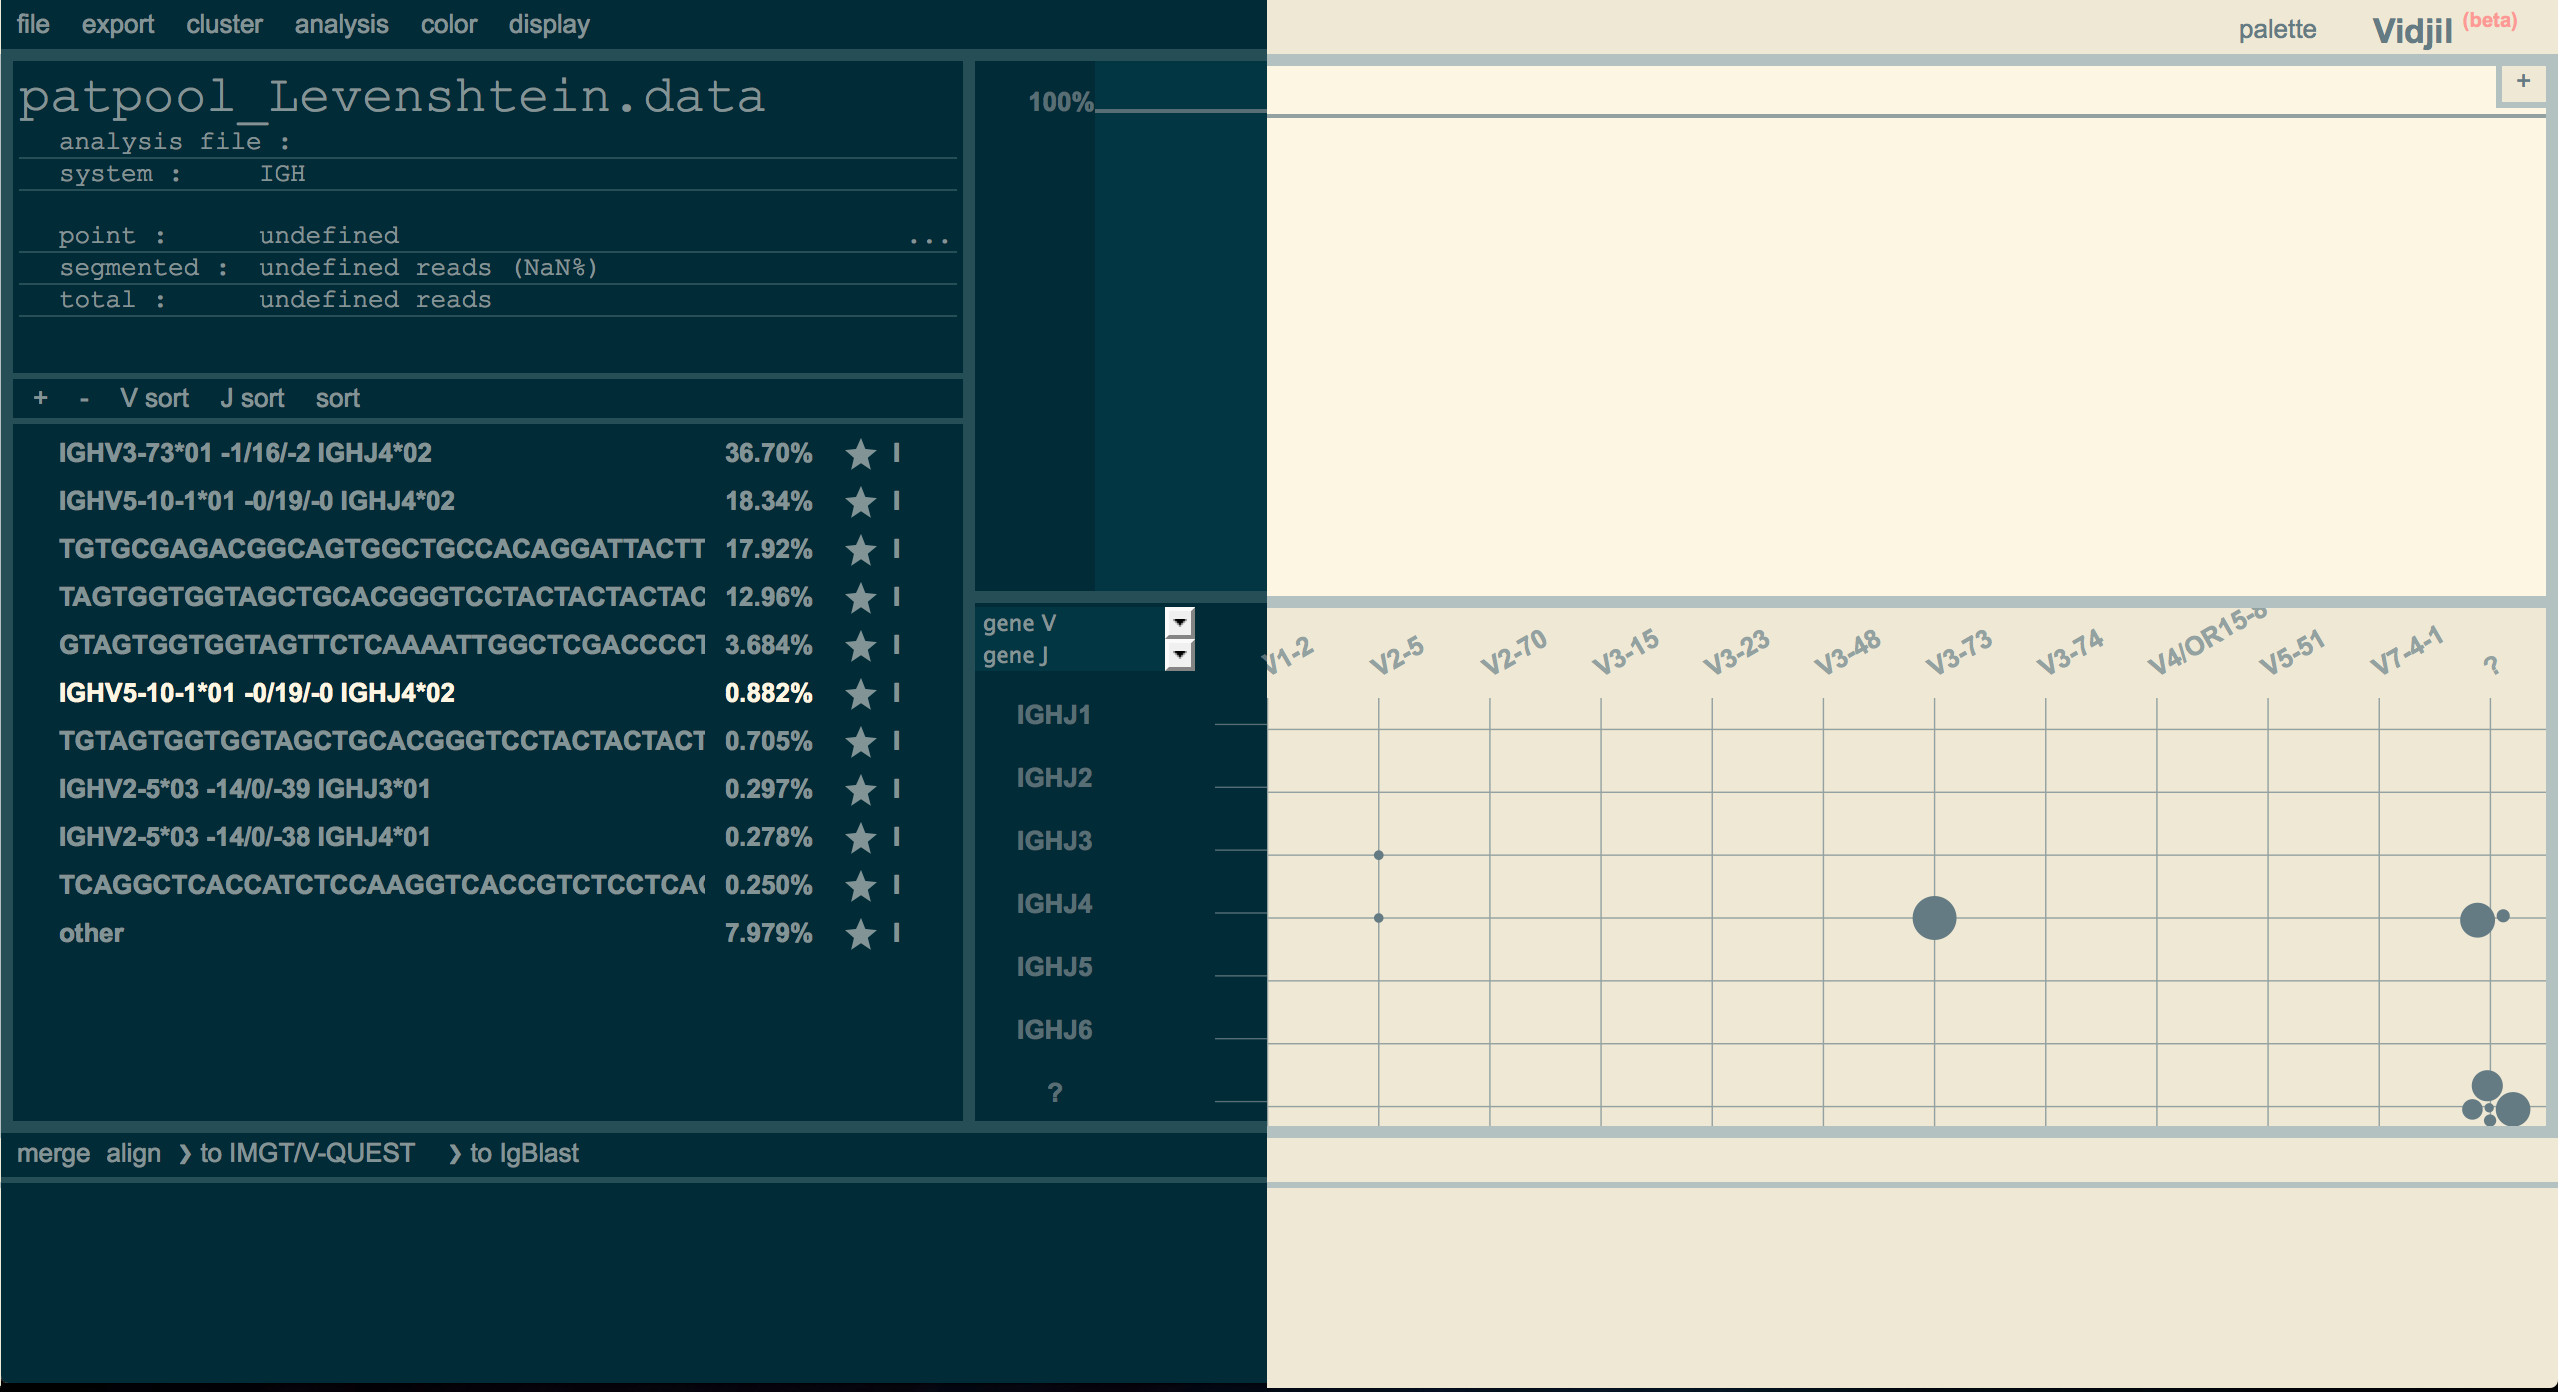
\includegraphics[scale=0.35]{img/Montage_Sans_Annotations.jpg}
}
\end{center}
\caption{Aperçu général de l'\textit{afficheur} - montage avec palette ``Dark'' et ``Light''}
\end{figure}

\begin{figure}[h]
\begin{center}
	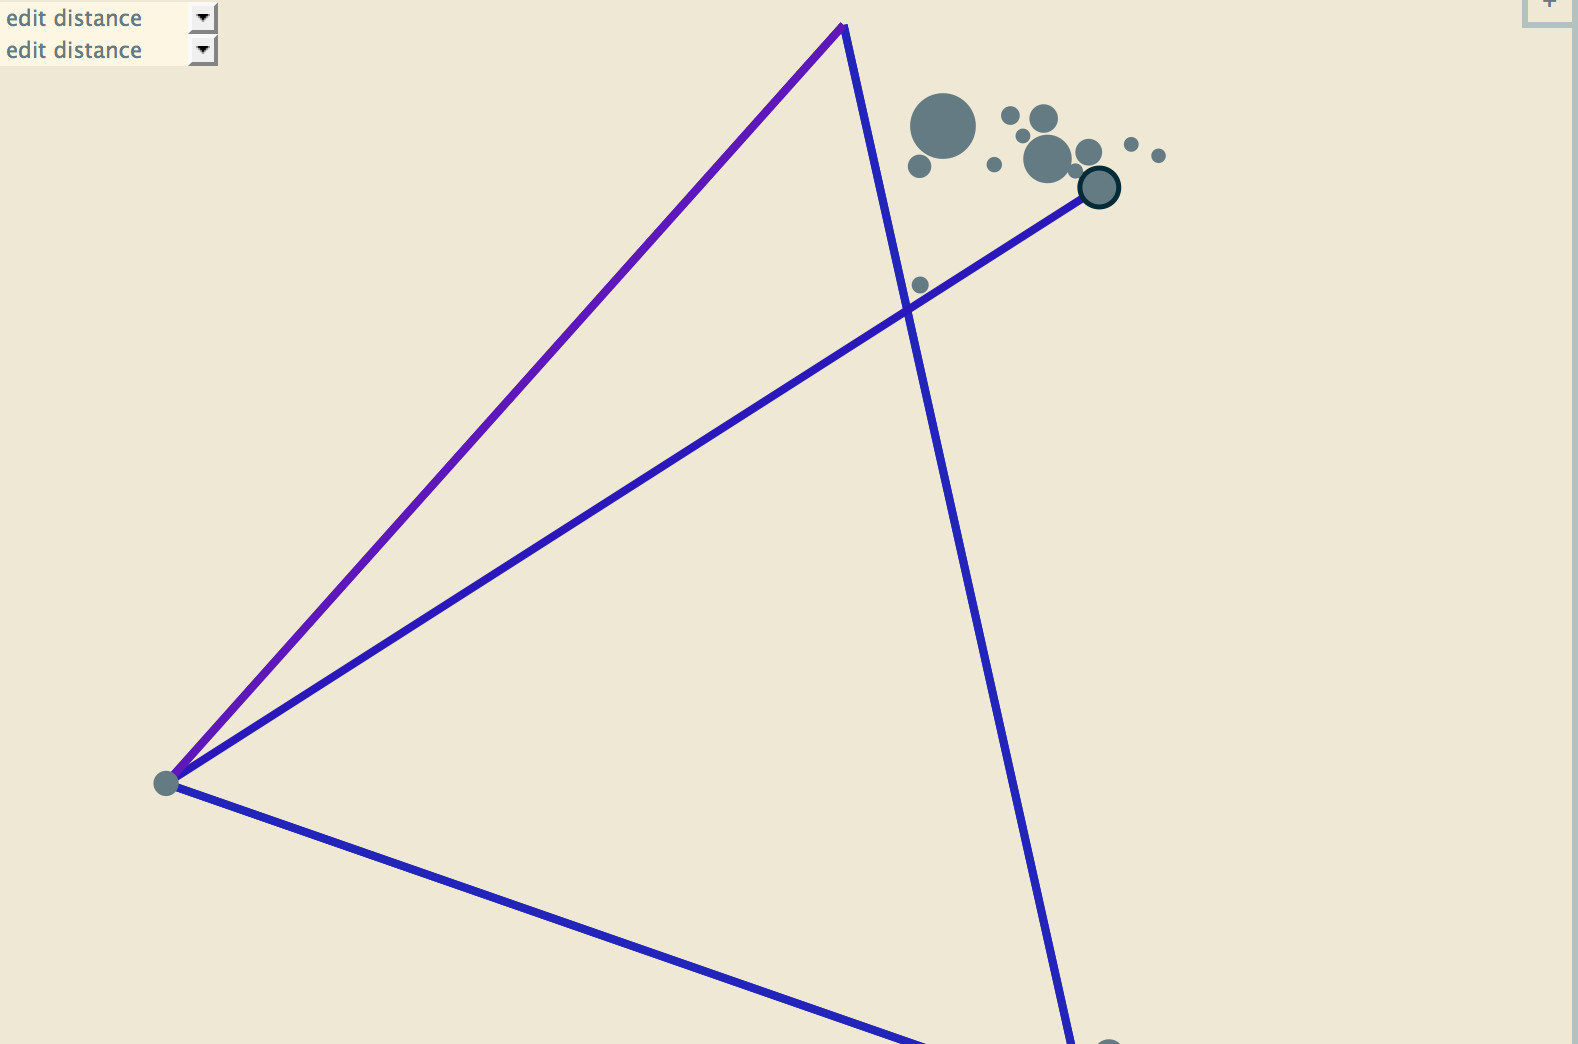
\includegraphics[scale=0.6]{img/Edit-Distance-Ex.jpg}
\end{center}
\caption{Aperçu général de l'\textit{afficheur} - montage avec palette ``Dark'' et ``Light''}
\end{figure}

\begin{pseudocode}{DBSCAN}{D, eps, MinPts}
\COMMENT{Base de l'algorithme}\\
C $=$ 0\\
$Pour chaque point $P$ non visité des données $D\\
$marquer $P$ comme visité$\\
PtsVoisins$ = $\CALL{epsilonVoisinage}{P, eps}\\
\IF tailleDe(PtsVoisins) < MinPts
\THEN $marquer $P$ comme "bruit"$
\ELSE 
	\BEGIN
		C$++$\\
		\CALL{extensionCluster}{D, P, PtsVoisins, C, eps, MinPts}\\
	\END\\
\\

\COMMENT{Procédure permettant d'inclure un point dans un cluster - extension d'un cluster}\\
\PROCEDURE {extensionCluster}{D, P, PtsVoisins, C, eps, MinPts}
	$Ajouter $P$ au cluster C$\\
	\FOREACH P' \in PtsVoisins \DO
			\IF P'$ n'a pas été visité$
			\THEN 
				\BEGIN
					$Marquer $P'$ comme visité$\\
					PtsVoisins'$ = $ \CALL{epsilonVoisinage}{D, P', eps}\\
					\IF tailleDe(PtsVoisins') >= MinPts
					\THEN PtsVoisins$ = $PtsVoisins \cup PtsVoisins'\\
				\END\\
			\IF P'$ n'est membre d'aucun cluster$
			\THEN $Ajouter $P'$ au cluster $C
\ENDPROCEDURE

\COMMENT{Procedure retournant tous les points de $D$ qui sont à une distance inférieure à $eps$ de $P$}\\
\PROCEDURE{epsilonVoisinage}{D, P, eps}
	$Retourner tous les points de $D$ qui sont à une distance inférieure à $eps$ de $P
\ENDPROCEDURE
\end{pseudocode}

\begin{figure}[h]
\begin{center}
\rotatebox{90}{
	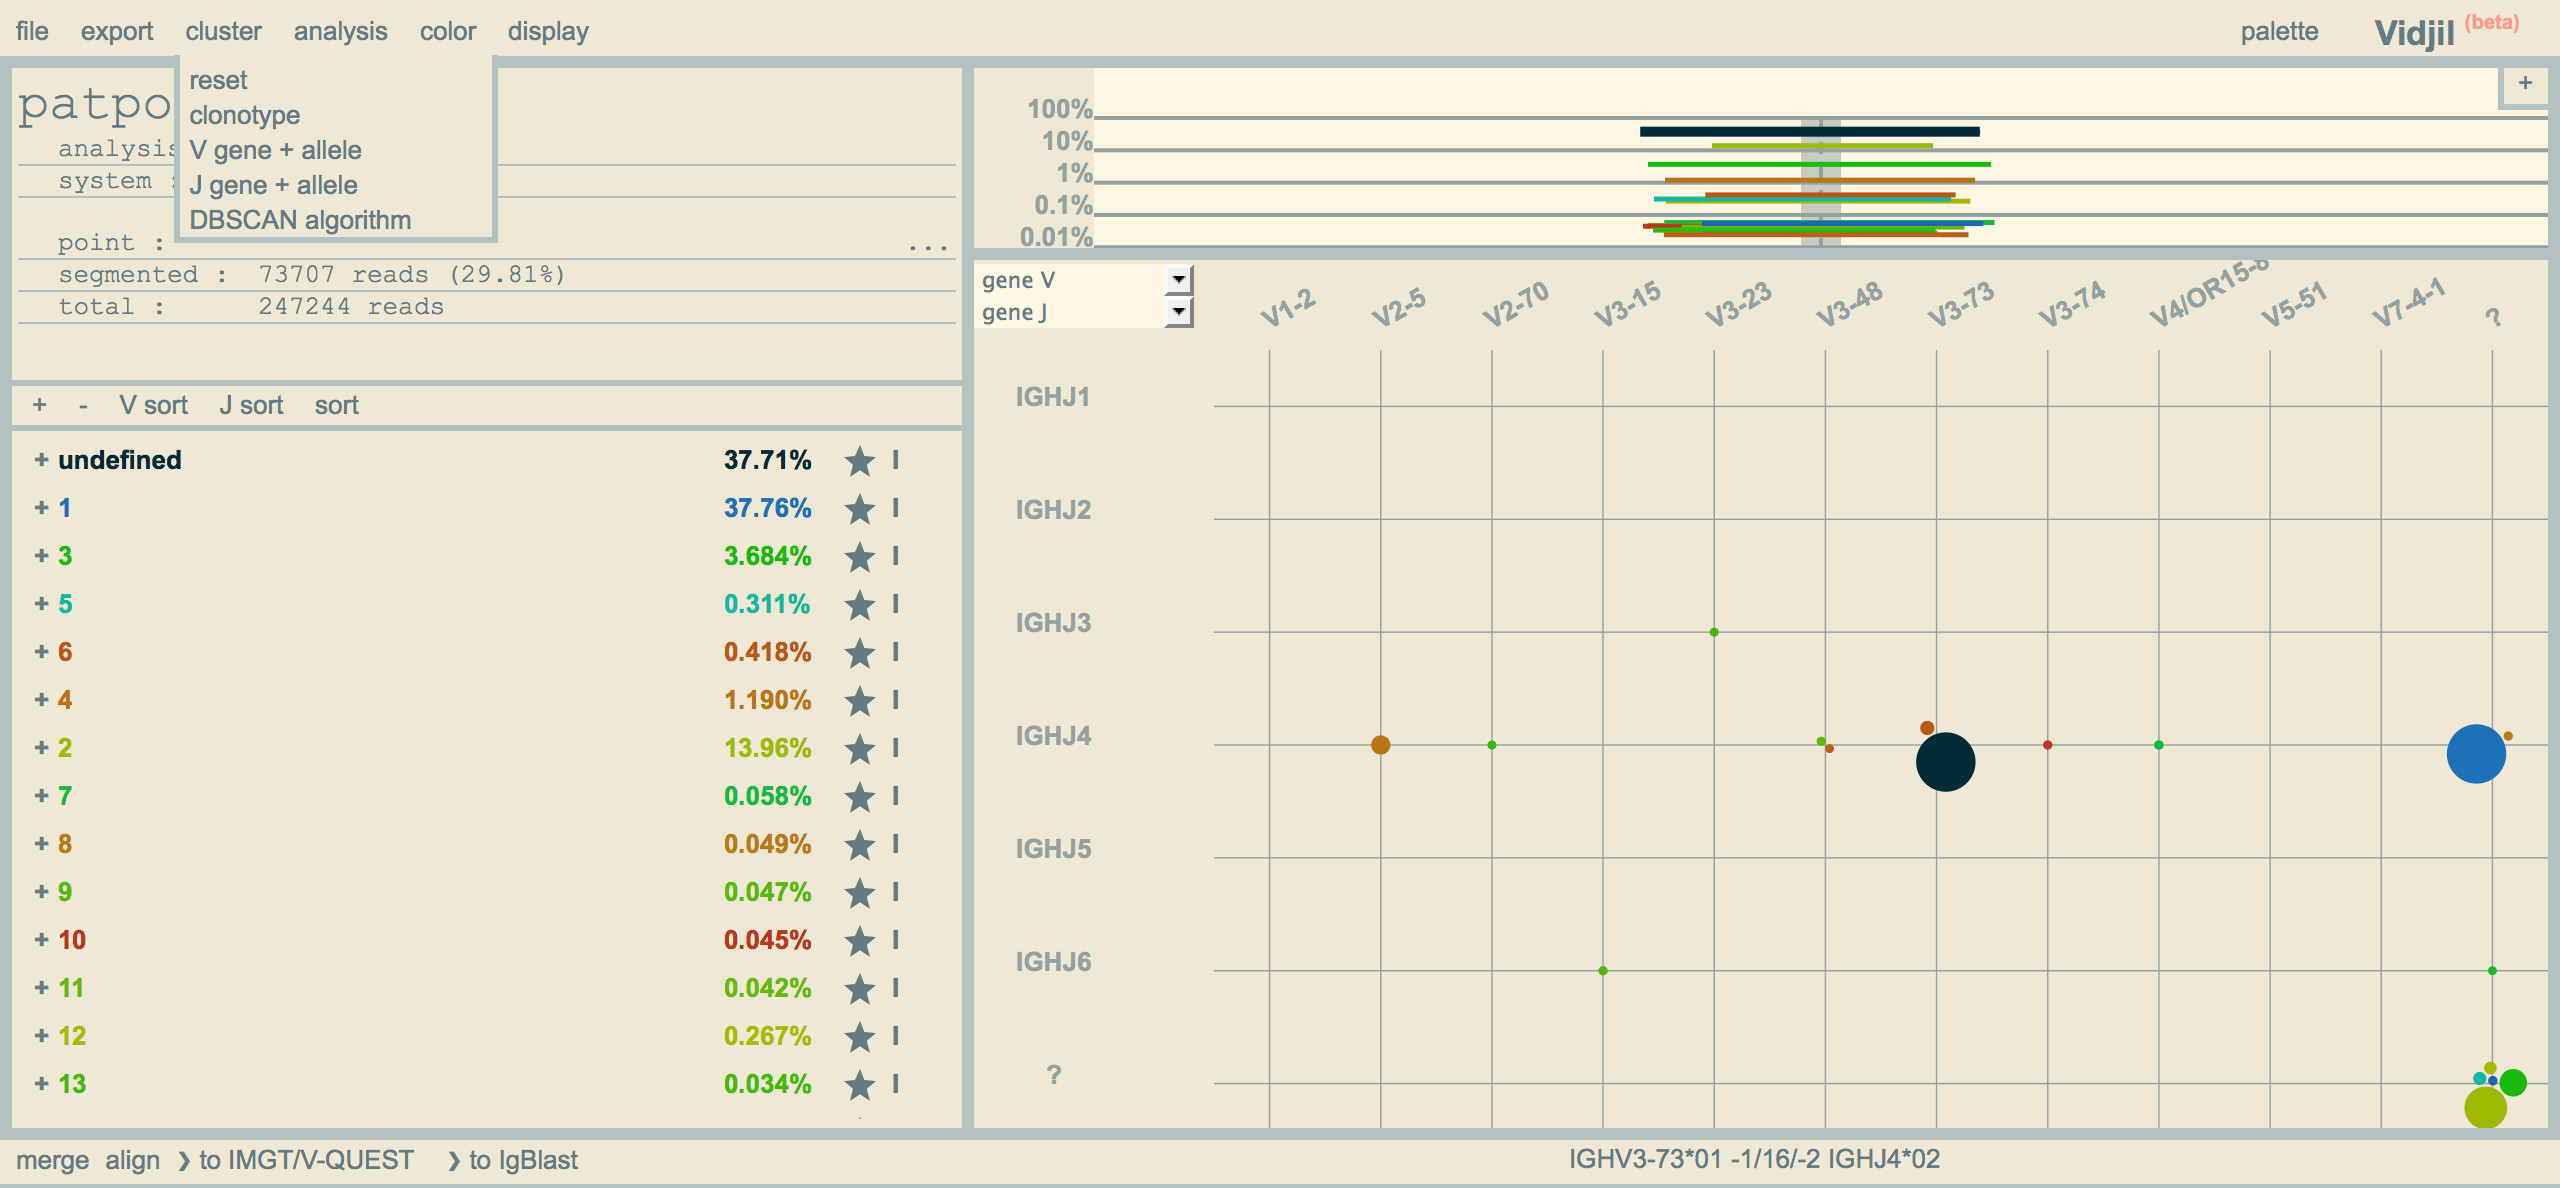
\includegraphics[scale=0.45]{img/DBSCAN-Cluster-Ex.jpg}
}
\end{center}
\caption{\textit{Afficheur} avec la clusterisation DBSCAN}
\end{figure}

\begin{figure}[h]
\begin{center}
\rotatebox{90}{
	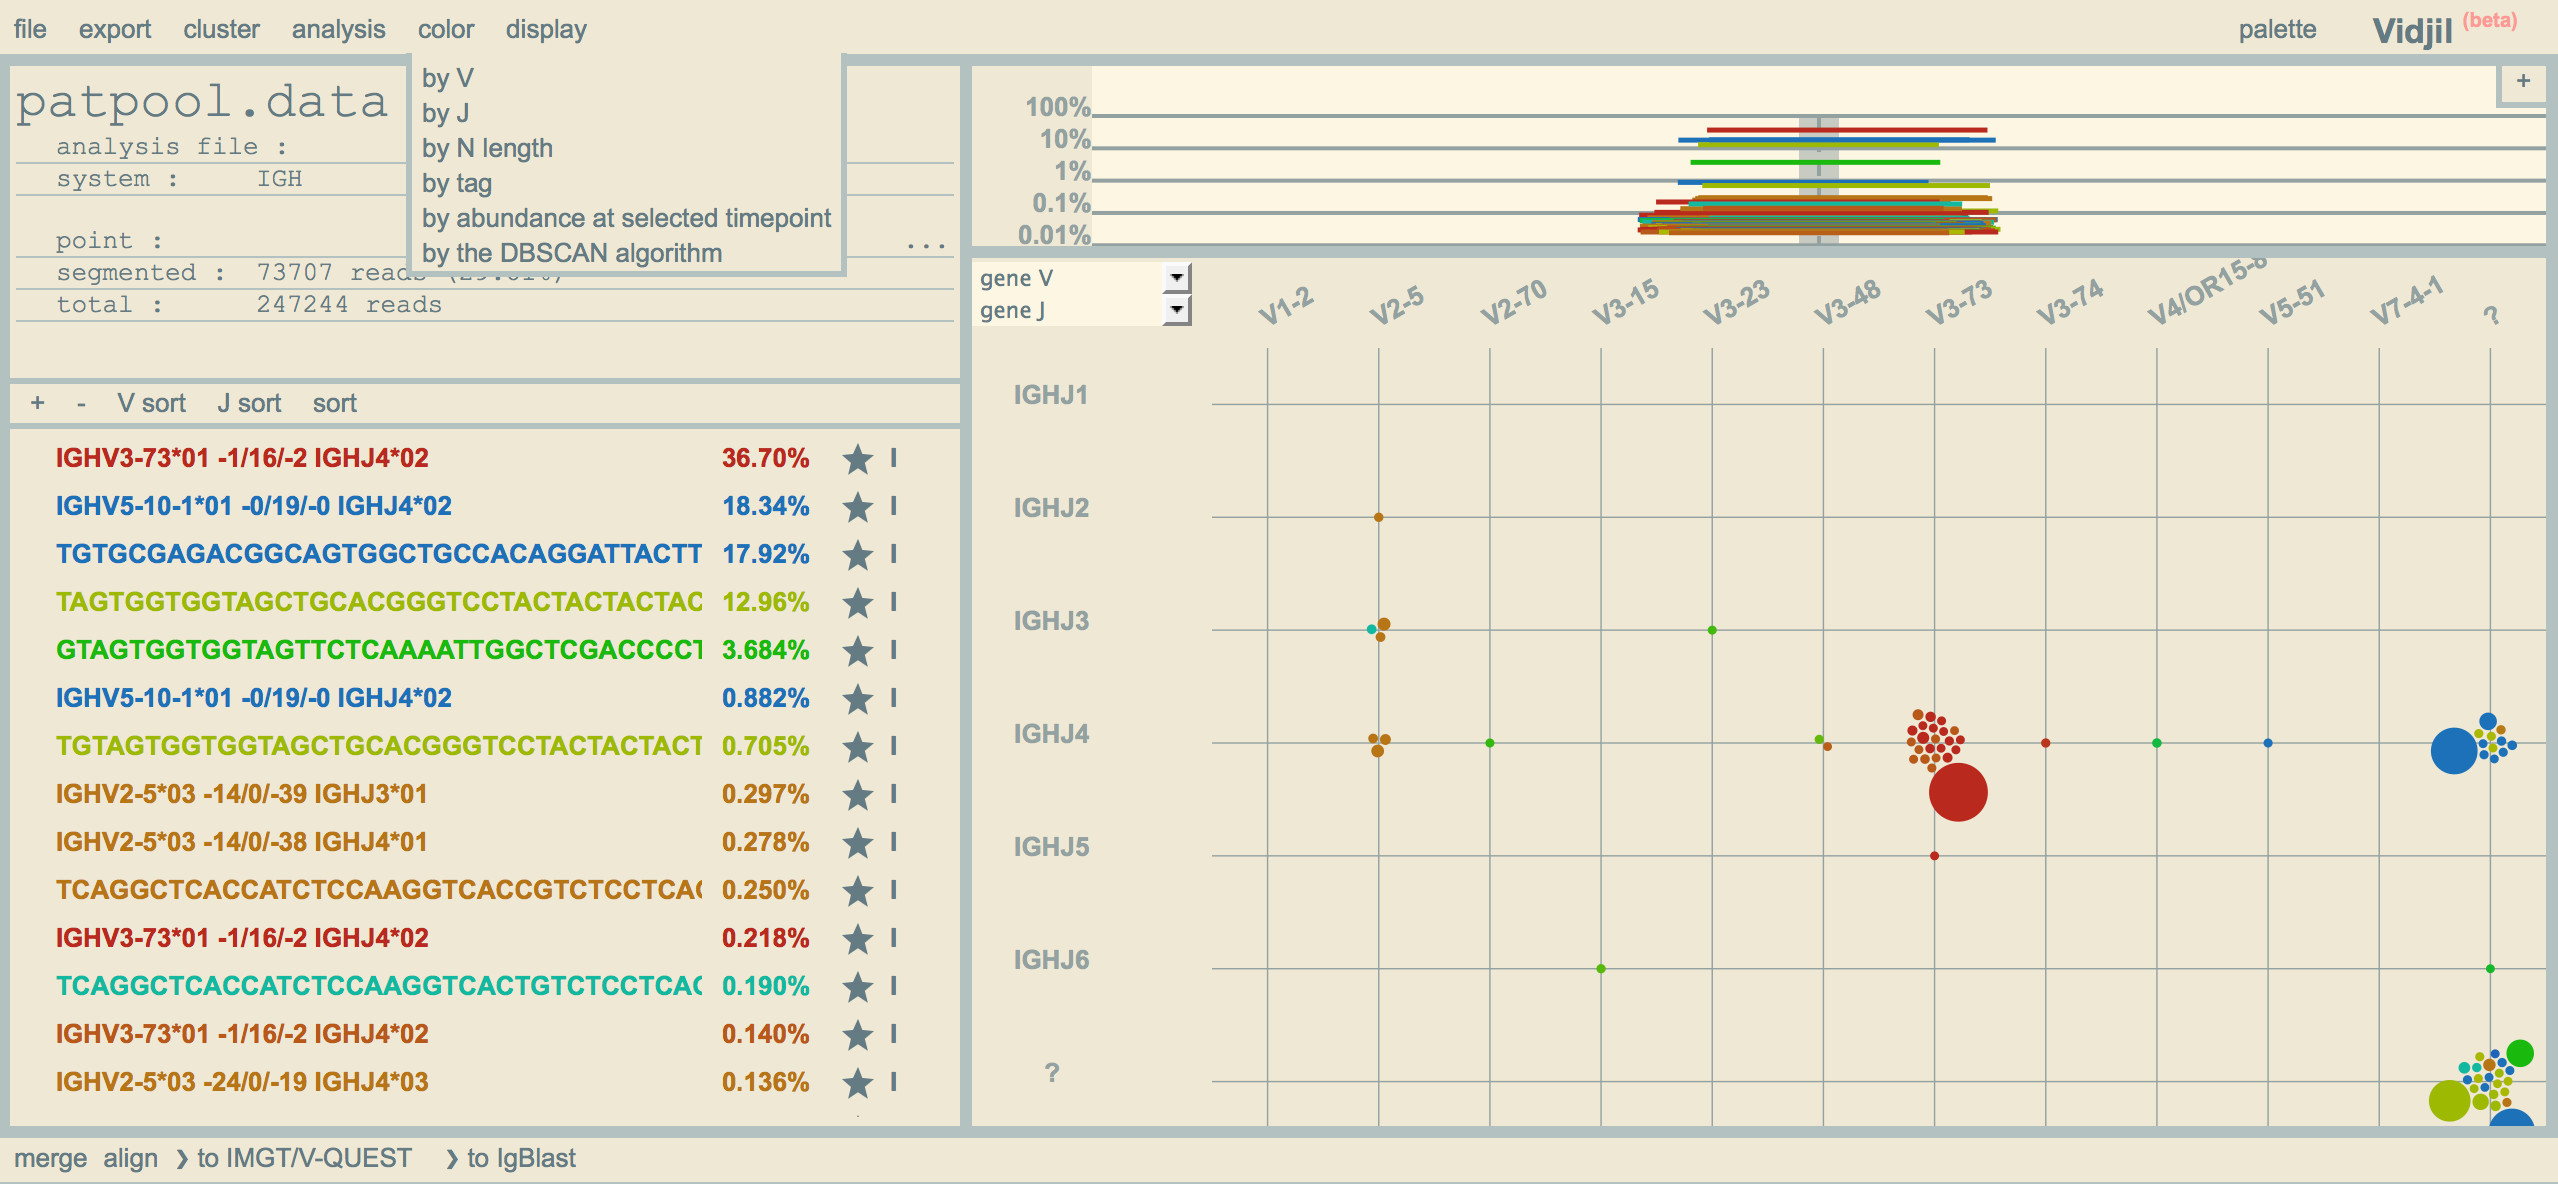
\includegraphics[scale=0.45]{img/DBSCAN-Color-Ex.jpg}
}
\end{center}
\caption{\textit{Afficheur} avec la colorisation DBSCAN}
\end{figure}

\begin{figure}[h]
\begin{center}
	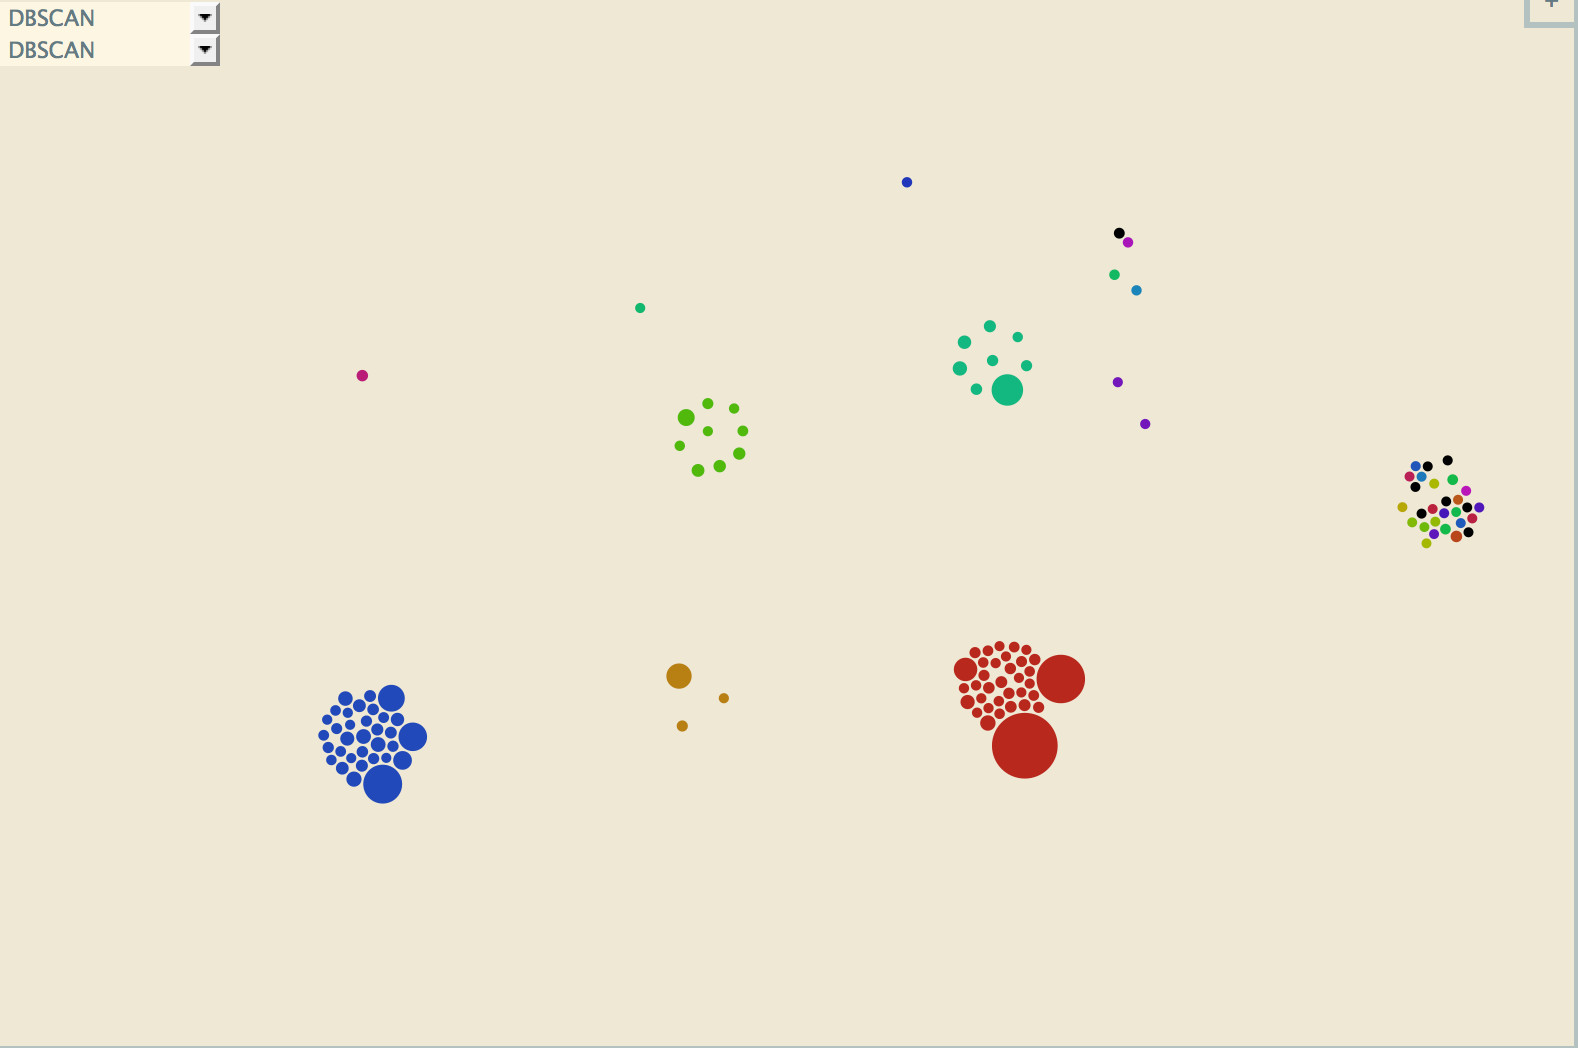
\includegraphics[scale=0.6]{img/DBSCAN-Ex.jpg}
\end{center}
\caption{\textit{Afficheur} avec la distribution DBSCAN}
\end{figure}

\end{spacing}
\end{document}